\documentclass[border=8pt,multi=tikzpicture]{standalone}
\usepackage[utf8]{inputenc}
\usepackage{lmodern}
\usepackage{tikz}
\usepackage{xcolor}
\usepackage{amsmath,amssymb}
\usetikzlibrary{shapes.geometric,arrows.meta,positioning,fit,calc,
                shadows,backgrounds,decorations.pathreplacing,
                patterns,shapes.symbols,shapes.misc,trees}

\definecolor{udblue}{RGB}{0,51,102}
\definecolor{udred}{RGB}{179,0,0}
\definecolor{lowrisk}{RGB}{198,239,206}
\definecolor{medrisk}{RGB}{255,235,156}
\definecolor{highrisk}{RGB}{255,199,206}
\definecolor{critrisk}{RGB}{255,128,128}

\tikzset{
  service/.style={rectangle, rounded corners=3pt, draw=udblue, fill=udblue!10,
                  thick, minimum width=2.0cm, minimum height=0.8cm,
                  align=center, font=\scriptsize\sffamily},
  data/.style={cylinder, shape border rotate=90, aspect=0.25, draw=udblue,
               fill=udblue!8, thick, minimum width=1.5cm, minimum height=1.0cm,
               align=center, font=\scriptsize\sffamily},
  client/.style={rectangle, rounded corners=2pt, draw=udred, fill=udred!10,
                 thick, minimum width=1.6cm, minimum height=0.6cm,
                 align=center, font=\scriptsize\sffamily},
  external/.style={rectangle, dashed, draw=black!60, fill=gray!10,
                   thick, minimum width=1.6cm, minimum height=0.6cm,
                   align=center, font=\scriptsize\sffamily},
  arrow/.style={-Stealth, thick, draw=udblue!70},
  process/.style={rectangle, rounded corners=2pt, draw=udblue, fill=udblue!8,
                  thick, minimum width=2.4cm, minimum height=0.7cm,
                  align=center, font=\scriptsize\sffamily}
}

\begin{document}
% This file is compiled once per diagram by passing \def\Diagram{N}
% via -jobname. We instead emit all diagrams as separate pages of one
% standalone PDF via \standaloneenv{tikzpicture} multipage.

% Diagram 1 - Architecture
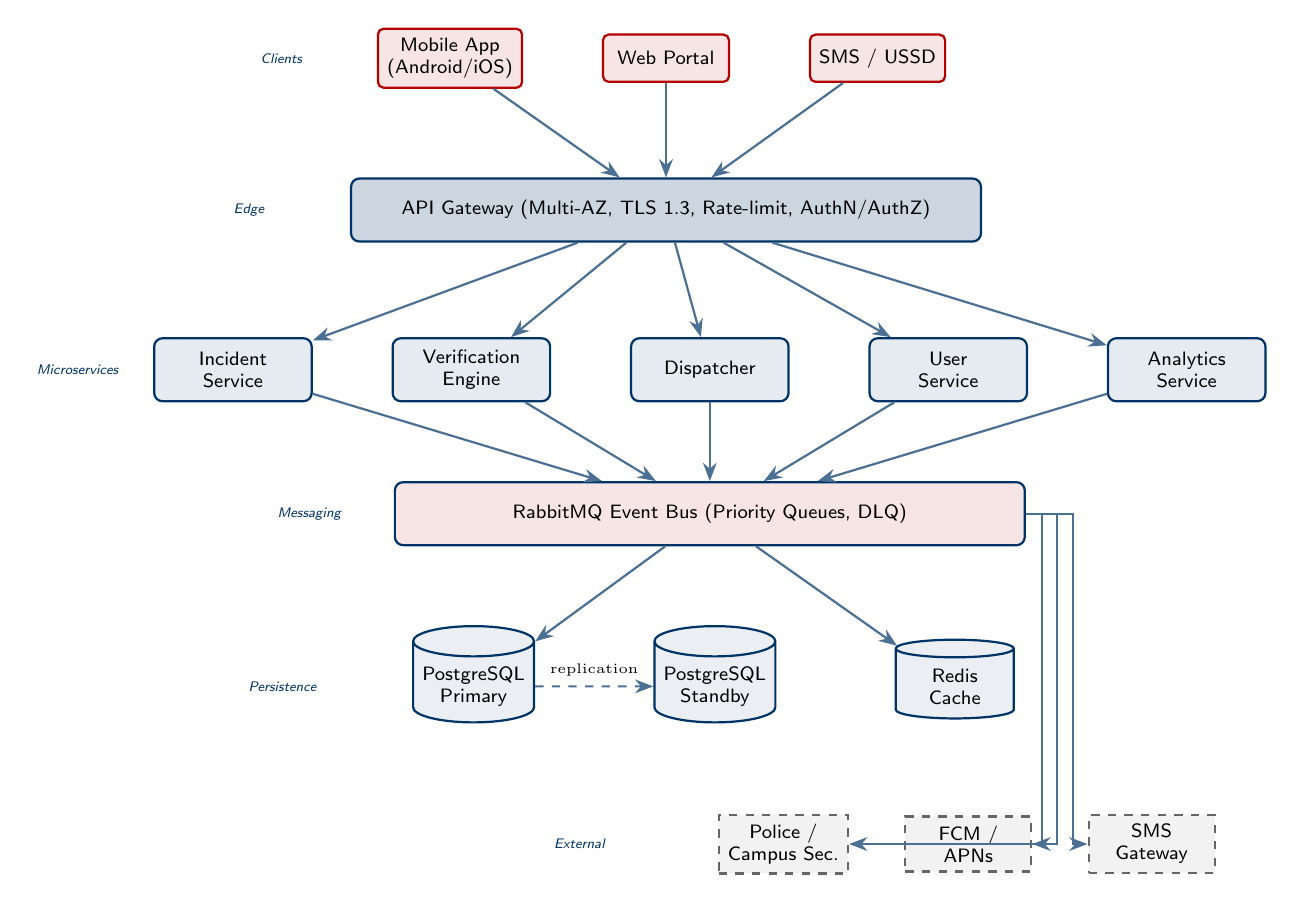
\begin{tikzpicture}[node distance=0.9cm and 1.0cm]
\node[client] (mobile) {Mobile App\\(Android/iOS)};
\node[client, right=of mobile] (web) {Web Portal};
\node[client, right=of web] (sms) {SMS / USSD};
\node[service, below=1.2cm of web, minimum width=8cm, fill=udblue!20] (gw)
  {API Gateway (Multi-AZ, TLS 1.3, Rate-limit, AuthN/AuthZ)};
\node[service, below=1.2cm of gw, xshift=-5.5cm] (incident) {Incident\\Service};
\node[service, right=of incident] (verif) {Verification\\Engine};
\node[service, right=of verif] (disp) {Dispatcher};
\node[service, right=of disp] (user) {User\\Service};
\node[service, right=of user] (analytics) {Analytics\\Service};
\node[service, below=1.0cm of disp, minimum width=8cm, fill=udred!10]
  (mq) {RabbitMQ Event Bus (Priority Queues, DLQ)};
\node[data, below=1.0cm of mq, xshift=-3cm] (pg) {PostgreSQL\\Primary};
\node[data, right=1.5cm of pg] (pgsb) {PostgreSQL\\Standby};
\node[data, right=1.5cm of pgsb] (cache) {Redis\\Cache};
\node[external, below=1.2cm of cache, xshift=2.5cm] (smsgw) {SMS\\Gateway};
\node[external, left=0.7cm of smsgw] (push) {FCM /\\APNs};
\node[external, left=0.7cm of push] (auth) {Police /\\Campus Sec.};
\draw[arrow] (mobile) -- (gw);
\draw[arrow] (web) -- (gw);
\draw[arrow] (sms) -- (gw);
\draw[arrow] (gw) -- (incident);
\draw[arrow] (gw) -- (verif);
\draw[arrow] (gw) -- (disp);
\draw[arrow] (gw) -- (user);
\draw[arrow] (gw) -- (analytics);
\draw[arrow] (incident) -- (mq);
\draw[arrow] (verif) -- (mq);
\draw[arrow] (disp) -- (mq);
\draw[arrow] (user) -- (mq);
\draw[arrow] (analytics) -- (mq);
\draw[arrow] (mq) -- (pg);
\draw[arrow, dashed] (pg) -- node[midway, above, font=\tiny]{replication} (pgsb);
\draw[arrow] (mq) -- (cache);
\draw[arrow] (mq.east) -| ($(mq.east)+(0.6,0)$) |- (smsgw);
\draw[arrow] (mq.east) -| ($(mq.east)+(0.4,0)$) |- (push);
\draw[arrow] (mq.east) -| ($(mq.east)+(0.2,0)$) |- (auth);
\node[font=\tiny\sffamily\itshape, anchor=west, text=udblue]
  at ($(mobile.west)+(-1.6,0)$) {Clients};
\node[font=\tiny\sffamily\itshape, anchor=west, text=udblue]
  at ($(gw.west)+(-1.6,0)$) {Edge};
\node[font=\tiny\sffamily\itshape, anchor=west, text=udblue]
  at ($(incident.west)+(-1.6,0)$) {Microservices};
\node[font=\tiny\sffamily\itshape, anchor=west, text=udblue]
  at ($(mq.west)+(-1.6,0)$) {Messaging};
\node[font=\tiny\sffamily\itshape, anchor=west, text=udblue]
  at ($(pg.west)+(-2.2,0)$) {Persistence};
\node[font=\tiny\sffamily\itshape, anchor=west, text=udblue]
  at ($(auth.west)+(-2.2,0)$) {External};
\end{tikzpicture}

% Diagram 2 - QA pipeline
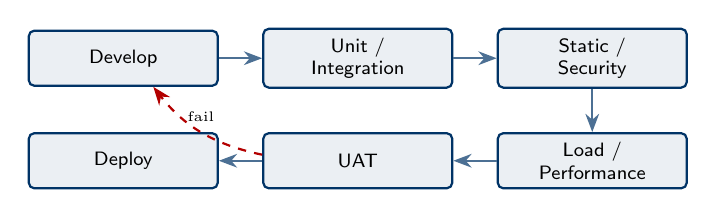
\begin{tikzpicture}[node distance=0.55cm and 0.55cm]
\node[process] (dev) {Develop};
\node[process, right=of dev] (unit) {Unit /\\Integration};
\node[process, right=of unit] (sec) {Static /\\Security};
\node[process, below=of sec] (load) {Load /\\Performance};
\node[process, left=of load] (uat) {UAT};
\node[process, left=of uat] (deploy) {Deploy};
\draw[arrow] (dev) -- (unit);
\draw[arrow] (unit) -- (sec);
\draw[arrow] (sec) -- (load);
\draw[arrow] (load) -- (uat);
\draw[arrow] (uat) -- (deploy);
\draw[arrow, dashed, draw=udred] (uat) to[bend left=20]
  node[midway,above,font=\tiny]{fail} (dev);
\end{tikzpicture}

% Diagram 3 - Risk Heat Map
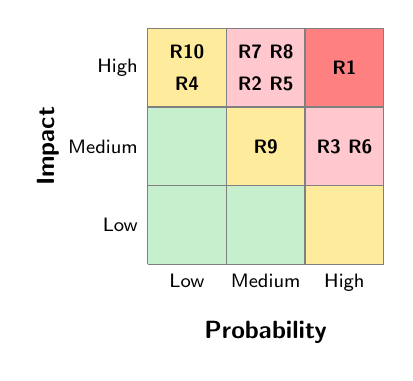
\begin{tikzpicture}[scale=1.0, every node/.style={font=\scriptsize\sffamily}]
\foreach \x/\y/\col in {
  0/0/lowrisk,  1/0/lowrisk,  2/0/medrisk,
  0/1/lowrisk,  1/1/medrisk,  2/1/highrisk,
  0/2/medrisk,  1/2/highrisk, 2/2/critrisk}
  \fill[\col] (\x,\y) rectangle (\x+1,\y+1);
\draw[step=1.0, black!50] (0,0) grid (3,3);
\node[anchor=north] at (0.5,0) {Low};
\node[anchor=north] at (1.5,0) {Medium};
\node[anchor=north] at (2.5,0) {High};
\node[anchor=east]  at (0,0.5) {Low};
\node[anchor=east]  at (0,1.5) {Medium};
\node[anchor=east]  at (0,2.5) {High};
\node[rotate=90, anchor=south, font=\small\bfseries\sffamily] at (-1.0,1.5) {Impact};
\node[anchor=north, font=\small\bfseries\sffamily] at (1.5,-0.6) {Probability};
\node at (0.5,2.3) {\textbf{R4}};
\node at (0.5,2.7) {\textbf{R10}};
\node at (1.5,1.5) {\textbf{R9}};
\node at (1.3,2.3) {\textbf{R2}};
\node at (1.7,2.3) {\textbf{R5}};
\node at (1.3,2.7) {\textbf{R7}};
\node at (1.7,2.7) {\textbf{R8}};
\node at (2.3,1.5) {\textbf{R3}};
\node at (2.7,1.5) {\textbf{R6}};
\node at (2.5,2.5) {\textbf{R1}};
\end{tikzpicture}

% Diagram 4 - Org chart

\begin{tikzpicture}[
  every node/.style={rectangle, rounded corners=2pt, draw=udblue, fill=udblue!10,
                     thick, minimum width=2.6cm, minimum height=0.7cm,
                     align=center, font=\scriptsize\sffamily},
  level distance=1.0cm, sibling distance=2.7cm,
  edge from parent/.style={draw=udblue!70, thick, -Stealth}]
\node {Project Manager}
  child {node {Architecture\\\& Quality Lead}}
  child {node {Risk\\Management Lead}}
  child {node {Implementation\\\& Evolution Lead}};
\end{tikzpicture}

% Diagram 5 - Gantt
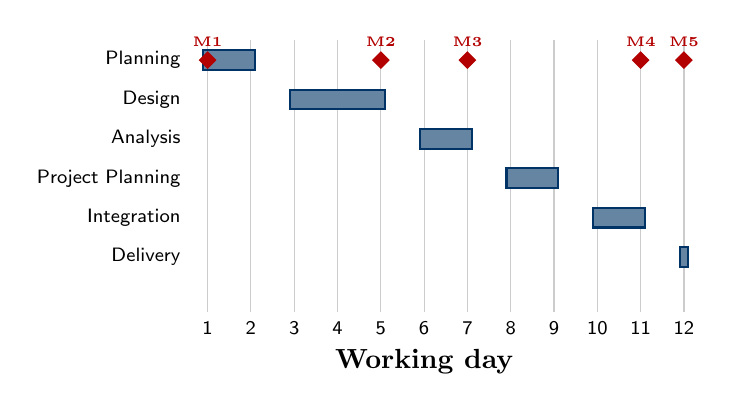
\begin{tikzpicture}[x=0.55cm, y=0.5cm, font=\scriptsize\sffamily]
\foreach \d in {1,...,12}
  \draw[gray!40] (\d,-0.4) -- (\d,6.5);
\foreach \d in {1,...,12}
  \node[anchor=north] at (\d,-0.4) {\d};
\node[anchor=north, font=\bfseries] at (6,-1.1) {Working day};
\foreach \name/\start/\end/\row in {
  Planning/1/2/6,
  Design/3/5/5,
  Analysis/6/7/4,
  Project Planning/8/9/3,
  Integration/10/11/2,
  Delivery/12/12/1}{
    \node[anchor=east] at (0.6,\row) {\name};
    \fill[udblue!60, draw=udblue, thick]
      (\start-0.1,\row-0.25) rectangle (\end+0.1,\row+0.25);
}
\foreach \day/\label in {1/M1, 5/M2, 7/M3, 11/M4, 12/M5}{
  \node[diamond, draw=udred, fill=udred, inner sep=1.5pt] at (\day,6) {};
  \node[anchor=south, font=\tiny\bfseries, text=udred] at (\day,6.1) {\label};
}
\end{tikzpicture}

% Diagram 6 - Deployment phases
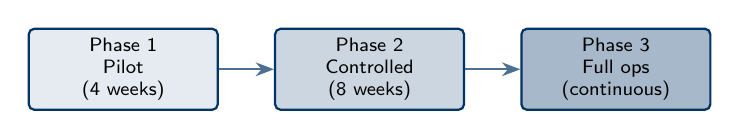
\begin{tikzpicture}[node distance=0.6cm and 0.7cm]
\node[process, fill=udblue!10] (p1) {Phase 1\\Pilot\\(4 weeks)};
\node[process, right=of p1, fill=udblue!20] (p2) {Phase 2\\Controlled\\(8 weeks)};
\node[process, right=of p2, fill=udblue!35] (p3) {Phase 3\\Full ops\\(continuous)};
\draw[arrow] (p1) -- (p2);
\draw[arrow] (p2) -- (p3);
\end{tikzpicture}

\end{document}
